\documentclass[titlepage,11pt]{article}
\usepackage{comment}
\usepackage{enumitem}
\usepackage{transparent} % Untuk transparansi gambar
\usepackage{listings}
\usepackage{amsmath}
\usepackage{graphicx}
\usepackage[font=small,labelfont=bf]{caption}
\usepackage[bahasa]{babel}
\usepackage{float}
\usepackage{verbatim}
\usepackage{graphicx,tabularx,multirow}
\usepackage{xcolor}
\usepackage[onehalfspacing]{setspace}
\usepackage[
	allcolors=visigrey,
	colorlinks=true,
]{hyperref}
\usepackage[a4paper,left=2cm,right=2cm]{geometry}
% Pengaturan kutipan artikel
\usepackage[style=ieee, backend=biber]{biblatex}
%Code listing style pak akok
\definecolor{codegreen}{rgb}{0,0.6,0}
\definecolor{codegray}{rgb}{0.5,0.5,0.5}
\definecolor{codepurple}{rgb}{0.58,0,0.82}
\definecolor{backcolour}{rgb}{0.95,0.95,0.92}

\usepackage{eso-pic} % Untuk menambahkan elemen ke seluruh halaman

\newcommand\BackgroundPic{
  \put(0,0){
    \parbox[b][\paperheight]{\paperwidth}{
      \vfill
      \centering
      \transparent{0.1}
      
\includegraphics[width=0.4\paperwidth,keepaspectratio]{miot.png}
      \vfill
    }
  }
}

\newcommand\BackgroundAllPages{ \AddToShipoutPicture*{\BackgroundPic} }
\newcommand\BackgroundNone{ \ClearShipoutPicture } % hilangkan background

\lstdefinestyle{mystyle}{
	backgroundcolor=\color{backcolour}, commentstyle=\color{codegreen},
	keywordstyle=\color{magenta},
	numberstyle=\small\color{codegray},
	stringstyle=\color{codepurple},
	basicstyle=\ttfamily\footnotesize,
	breakatwhitespace=false,         
	breaklines=true,                 
	captionpos=t,                    
	keepspaces=true,                 
	numbers=left,                    
	numbersep=5pt,                  
	showspaces=false,                
	showstringspaces=false,
	showtabs=false,           
	frame = single,
	tabsize=2
}
\lstset{style=mystyle}

\definecolor{visigrey}{rgb}{.1,.15,.15}
\geometry{top=1cm,bottom=.5cm}
\savegeometry{titlepage}
\geometry{top=2cm,bottom=2cm}
\savegeometry{main}

\def\bspace{\(\qquad\qquad\qquad\)}
\usepackage[T1]{fontenc}
\usepackage[utf8]{inputenc}
\usepackage{tgheros}
\renewcommand*\familydefault{\sfdefault}

\setcounter{tocdepth}{6}

\def\autor{Laboratorium }
\def\lab{Multimedia dan Internet of Things}
\def\departemen{Departemen Teknik Komputer}
\def\institut{Institut Teknologi Sepuluh Nopember}
\def\praktikum{Laporan Sementara \\ Praktikum Jaringan Komputer}
\def\nama{Muhammad Zidane Faiq Sidqi - 5024231040}
% Ubah Judul sesuai dengan modul
\def\judul{Firewall And NAT}
\def\tanggal{2025}
\begin{document}
% Ubah Bahasa sesuai dengan keinginan
\selectlanguage{bahasa}

\BackgroundNone
\def\headingtype{\bf \small}
\loadgeometry{titlepage}

\begin{titlepage}
	\centering
	\begin{tabularx}{\textwidth}{l@{\hskip 0pt}lX}
		\raisebox{-0.5\height}{
\includegraphics[width=3cm]{Cover/img/logodepart.png}} 
		& \raisebox{-0.5\height}{
\includegraphics[width=3cm]{Cover/img/miot.png}} 
		& \raggedleft
	\hfill
	\begin{minipage}{0.5\textwidth}
		\raggedleft
		{\emph{\headingtype \autor}} \\[-2pt]
		{\headingtype \lab} \\[-2pt]
		{\headingtype \departemen} \\[-2pt]
		{\headingtype \emph{\institut}}
	\end{minipage}

	\vspace{5cm}
	\end{tabularx}
	
	\vspace{5cm}
	{\Huge \bf \praktikum \par}
	
	\vspace{2cm}
	{\LARGE \bf \judul \par}
	
	\vspace{2cm}
	{\Large \nama \par}
	
	\vfill
	{\Large \tanggal \par}
	
	\vfill
	
\includegraphics[width=\textwidth]{Cover/img/footer.png}
\end{titlepage}

\loadgeometry{main}


\BackgroundAllPages
% Pilih Modul yang akan di build
\section{Langkah-Langkah Percobaan}
\subsection{Wireless Point to Point}
1. Aktifkan Interface Wireless Wlan 1 Masuk pada Menu Wireless lalu Wifi Interface lalu Klik interface Wlan 1 dan tekan tanda panah warna biru untuk enable Konfigurasikan untuk Router A Sebagai ( setelah double Klik pada interface wlan 1 masuk ke tab Wireless ) : Mode : Bridge ; SSID : PointToPoint 17.
\begin{figure}[H]
    \centering
    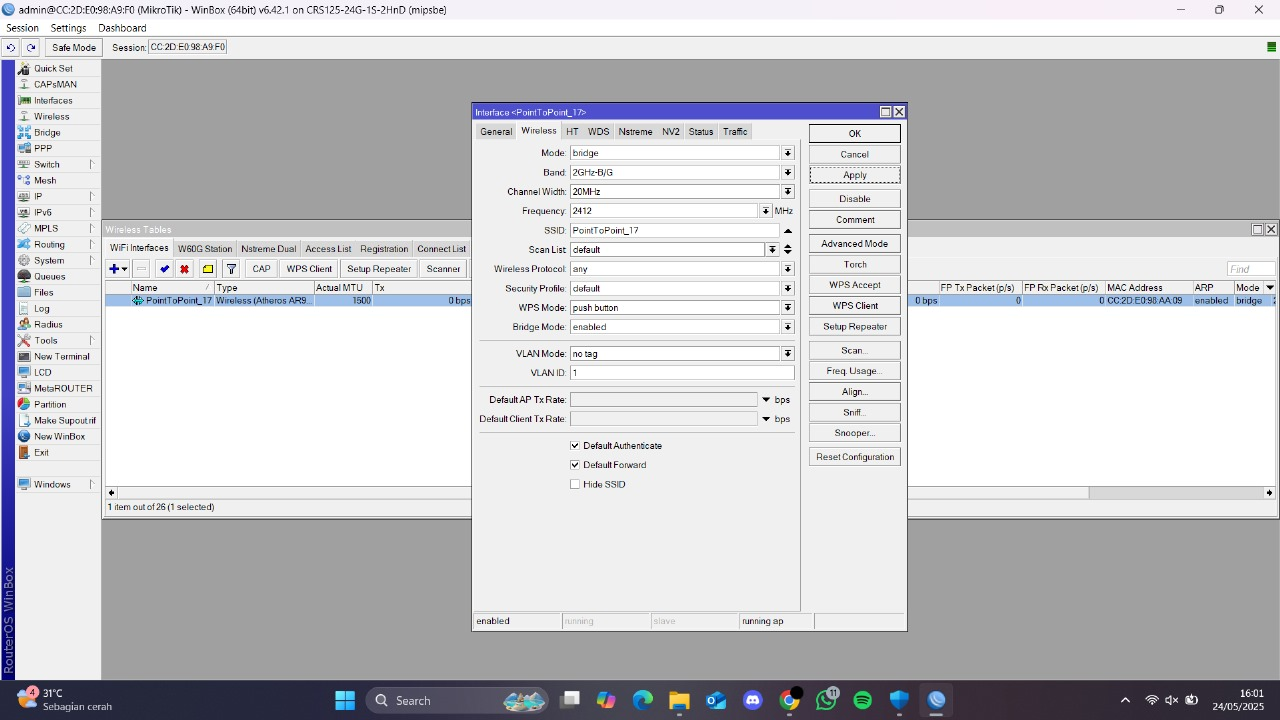
\includegraphics[width=0.65\linewidth]{image/bridge2.jpg}
    \label{fig:inirujukan}
    \caption{Konfigurasi router A}
\end{figure}
Konfigurasikan untuk Router B Sebagai ( setelah double Klik pada interface wlan 1 masuk ke tab Wireless ) : Mode : Station. Setelah itu klik tombol scan dan pilih interface menjadi wlan 1 lalu akan muncul berbagai jaringan wifi cari nama wifi yang sesuai dengan Router A lalu klik Connect.
\begin{figure}[H]
    \centering
    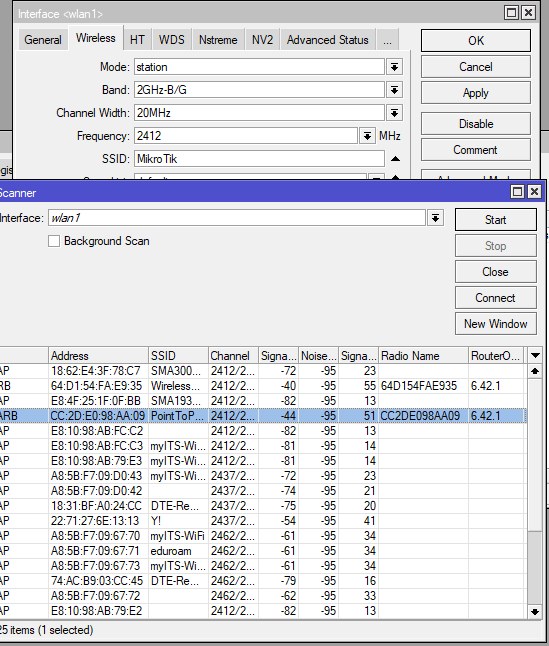
\includegraphics[width=0.65\linewidth]{image/bridge.png}
    \label{fig:inirujukan}
    \caption{Konfigurasi router B}
\end{figure}

2. Konfigurasi IP Address pada Wlan 1 Tambahkan IP address pada Wlan 1 yang digunakan sebagai jalur antar-router. Karena hanya ada dua perangkat yang terhubung (router A dan router B), IP Wlan 1 Router A : 10.10.10.1/29 ; IP Wlan 1 Router B : 10.10.10.2/29. \\
3. Konfigurasi IP Address untuk Jaringan LAN (note lakukan konfigurasi ini pada router A dan b) Tambahkan IP address pada ether 2 yang digunakan untuk menghubungkan Laptop dengan Router. IP ether 2 Router A : 192.168.20.1/24 ; IP ether 2 Router B : 192.168.30.1/24
\begin{figure}[H]
    \centering
    \begin{subfigure}[b]{0.3\linewidth}
      \centering
      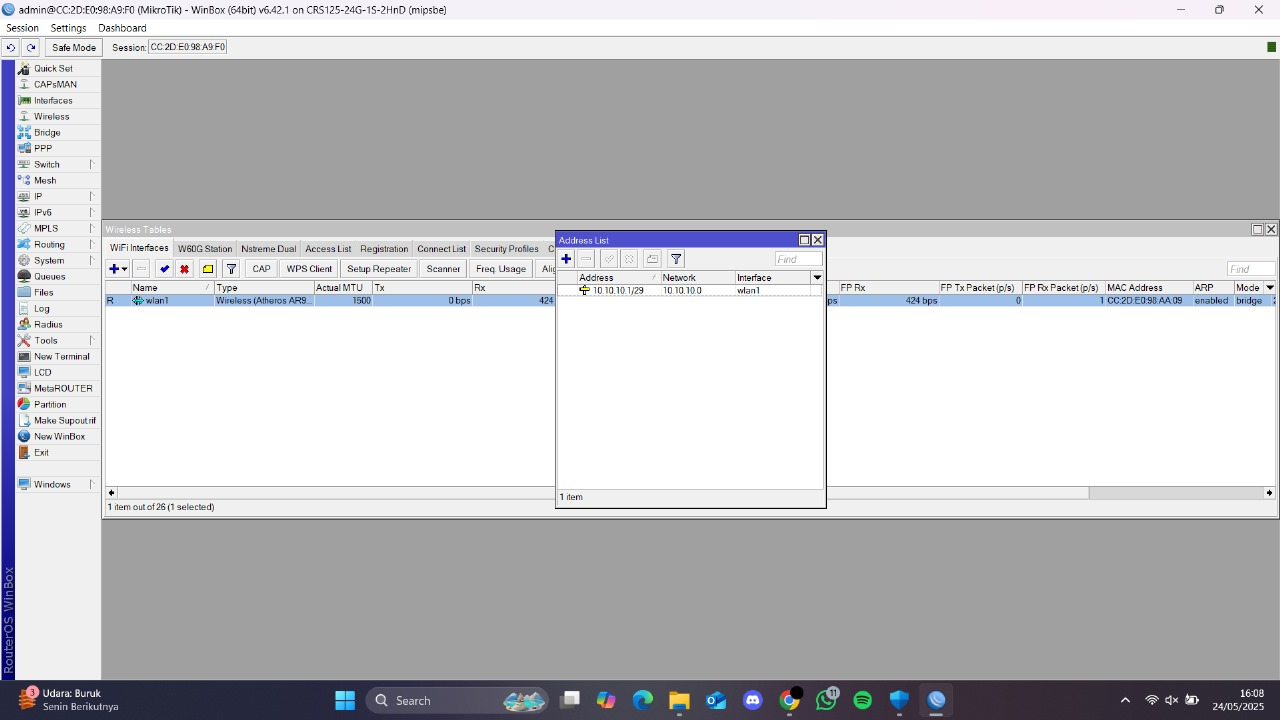
\includegraphics[width=\linewidth]{image/bridge4.jpg}
      \caption{router A}
    \end{subfigure}
    \hspace{1cm}
    \begin{subfigure}[b]{0.3\linewidth}
      \centering
      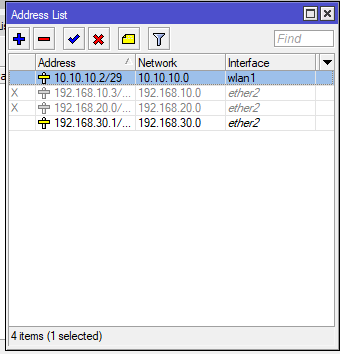
\includegraphics[width=\linewidth]{image/bridge1.png}
      \caption{router B}
    \end{subfigure}
    \caption{Konfigurasi Ip address wlan 1 dan ether 2}
\end{figure}

4. Konfigurasi Routing Statis (note lakukan konfigurasi ini pada router A dan b) Setelah semua interface diberi IP, langkah selanjutnya adalah menambahkan rute secara manual. Masuk ke menu IPv4 → Routes, kemudian klik "+" untuk menambahkan routing. Pada Router A, Dst. Address: 192.168.30.0/24 ; Gateway: 10.10.10.2. Pada Router B, Dst. Address: 192.168.20.0/24 ; Gateway: 10.10.10.1.
\begin{figure}[H]
    \centering
    \begin{subfigure}[b]{0.3\linewidth}
      \centering
      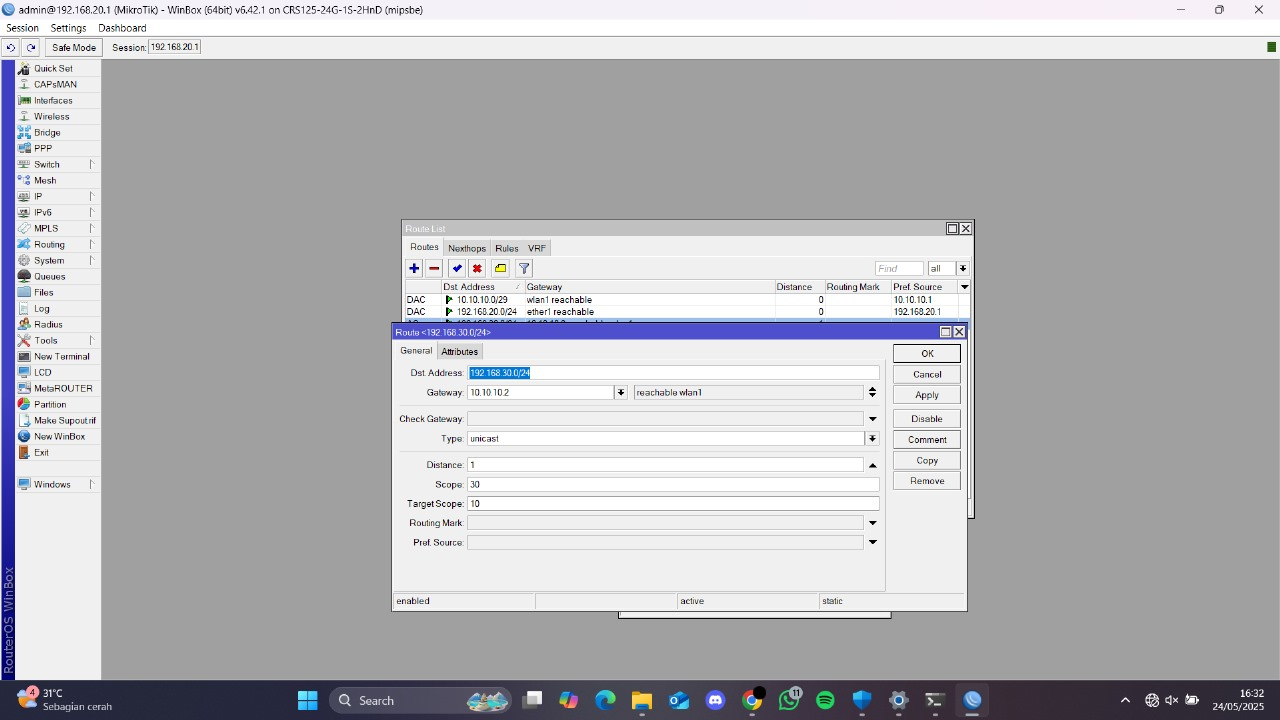
\includegraphics[width=\linewidth]{image/bridge6.jpg}
      \caption{router A}
    \end{subfigure}
    \hspace{1cm}
    \begin{subfigure}[b]{0.3\linewidth}
      \centering
      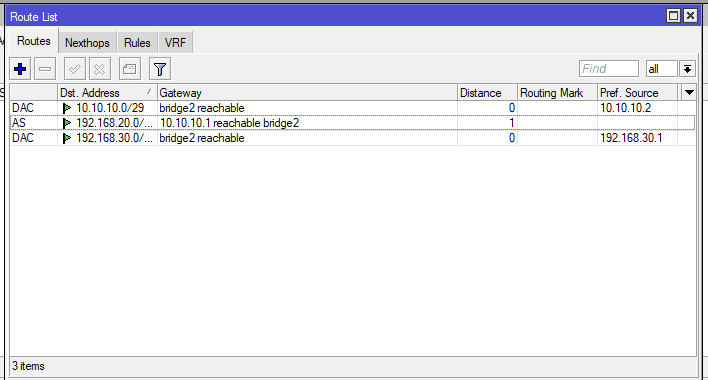
\includegraphics[width=\linewidth]{image/bridge3.png}
      \caption{router B}
    \end{subfigure}
    \caption{Konfigurasi routing statis}
\end{figure}

5. Test Koneksi Antar Router.
\begin{figure}[H]
    \centering
    \begin{subfigure}[b]{0.3\linewidth}
      \centering
      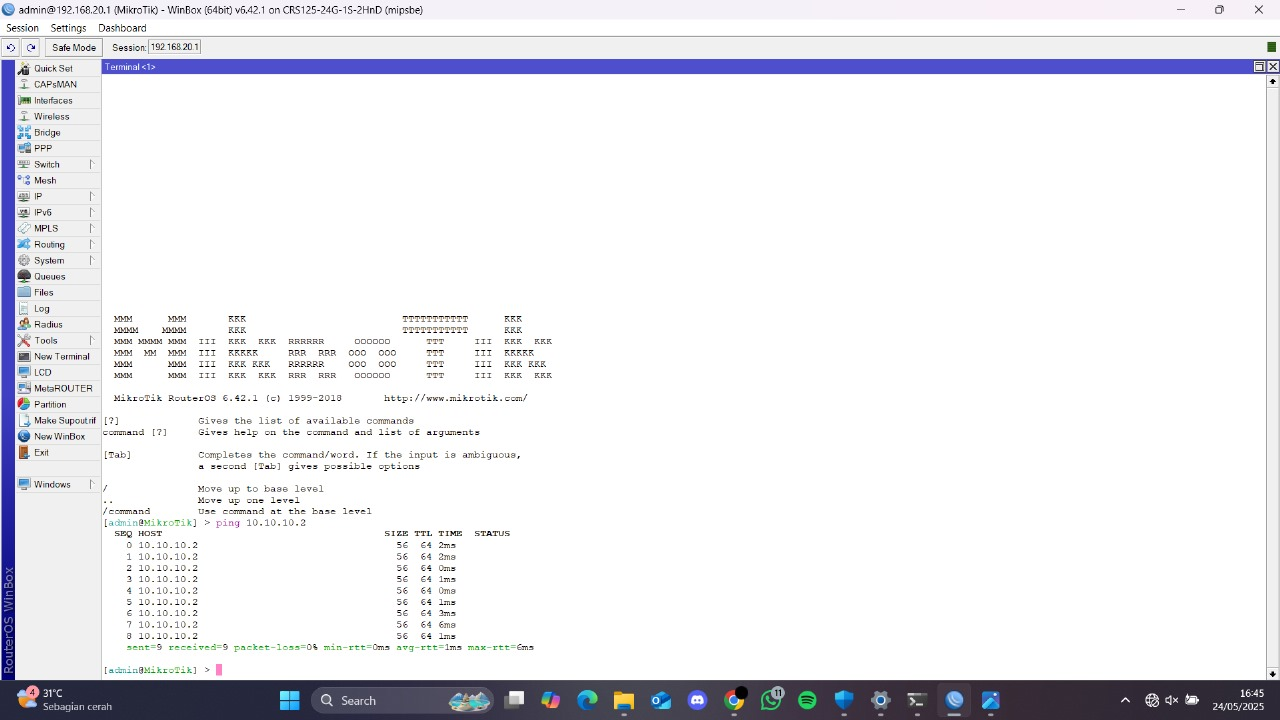
\includegraphics[width=\linewidth]{image/bridge8.jpg}
      \caption{router A}
    \end{subfigure}
    \hspace{1cm}
    \begin{subfigure}[b]{0.3\linewidth}
      \centering
      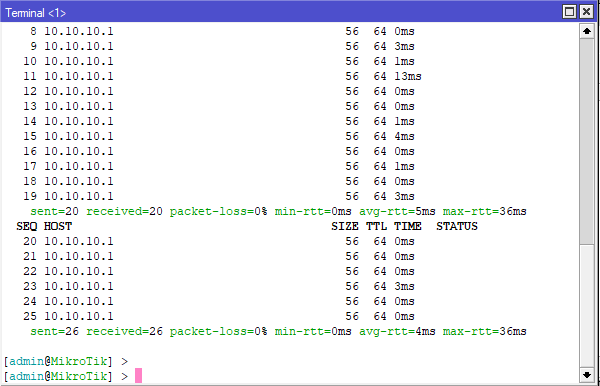
\includegraphics[width=\linewidth]{image/bridge5.png}
      \caption{router B}
    \end{subfigure}
    \caption{Ping terminal Winbox}
\end{figure}

6. Konfigurasi IP Adress di Laptop (note lakukan konfigurasi ini laptop yang terhubung pada router A dan b masing-masing) Karena ini masih menggunakan konfigurasi Static IP tambahkan IP address secara manual ke interface di laptop masing-masing bisa lewat Control Panel atau langsung di settings Windows, pastikan IP dan Gateway sudah benar sesuai Ether 2. Pada laptop yang terhubung ke Router A, IP Address : 192.168.20.2 ; Gateway : 192.168.20.1 (Router A) ; DNS : 8.8.8.8. Pada laptop yang terhubung ke Router B, IP Address: 192.168.30.2 ; Gateway : 192.168.30.1 (Router B) ; DNS : 8.8.8.8. 
\begin{figure}[H]
    \centering
    \begin{subfigure}[b]{0.3\linewidth}
      \centering
      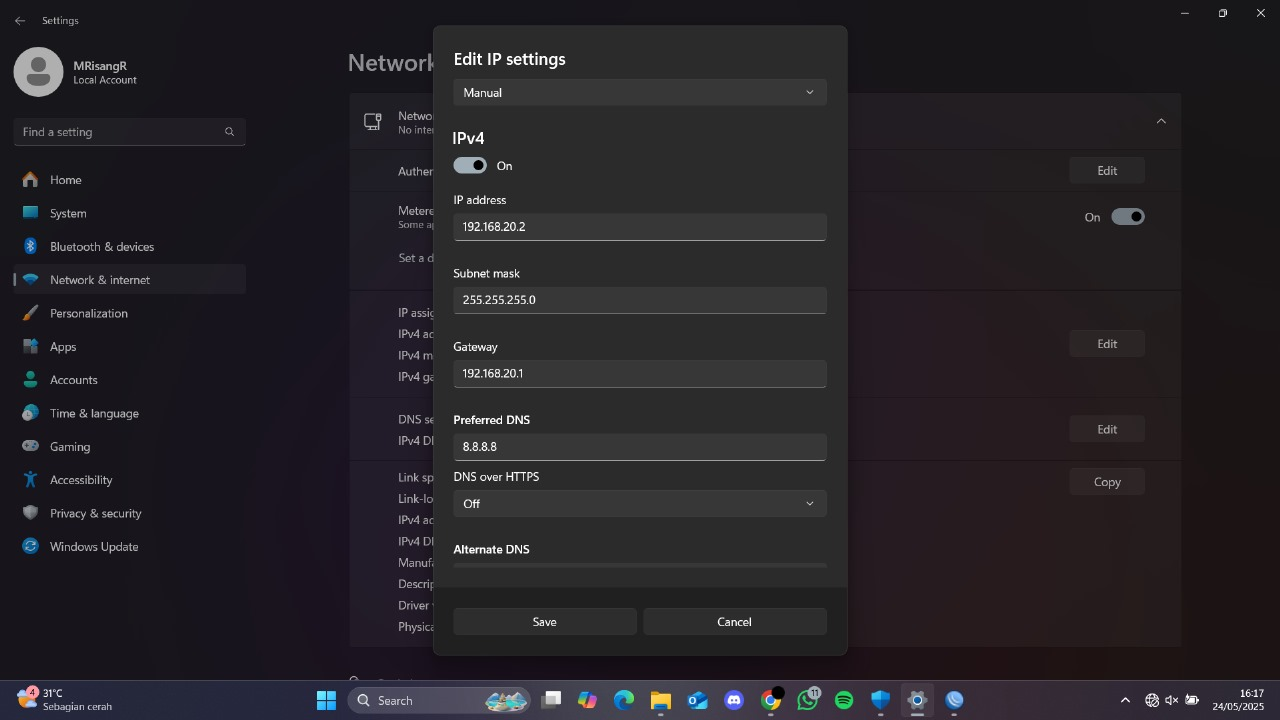
\includegraphics[width=\linewidth]{image/bridge10.jpg}
      \caption{Laptop 1}
    \end{subfigure}
    \hspace{1cm}
    \begin{subfigure}[b]{0.3\linewidth}
      \centering
      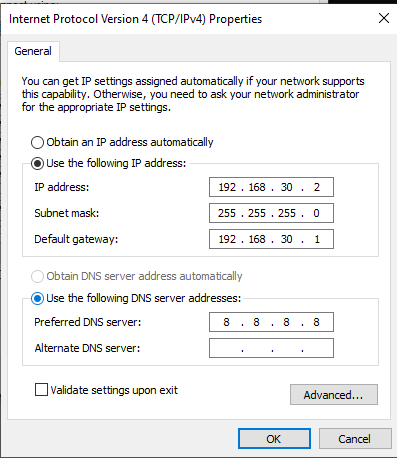
\includegraphics[width=\linewidth]{image/bridge7.png}
      \caption{Laptop 2}
    \end{subfigure}
    \caption{Ip address di masing-masing laptop}
\end{figure}

7. Jika Sudah Uji test PING dari Laptop 1 ke alamat Laptop 2, Jika berhasil maka Routing tidak ada masalah. Pada konfigurasikan Router B dan laptop yang terhubung ke Router B lakukan hal yang sama
\begin{figure}[H]
    \centering
    \begin{subfigure}[b]{0.3\linewidth}
      \centering
      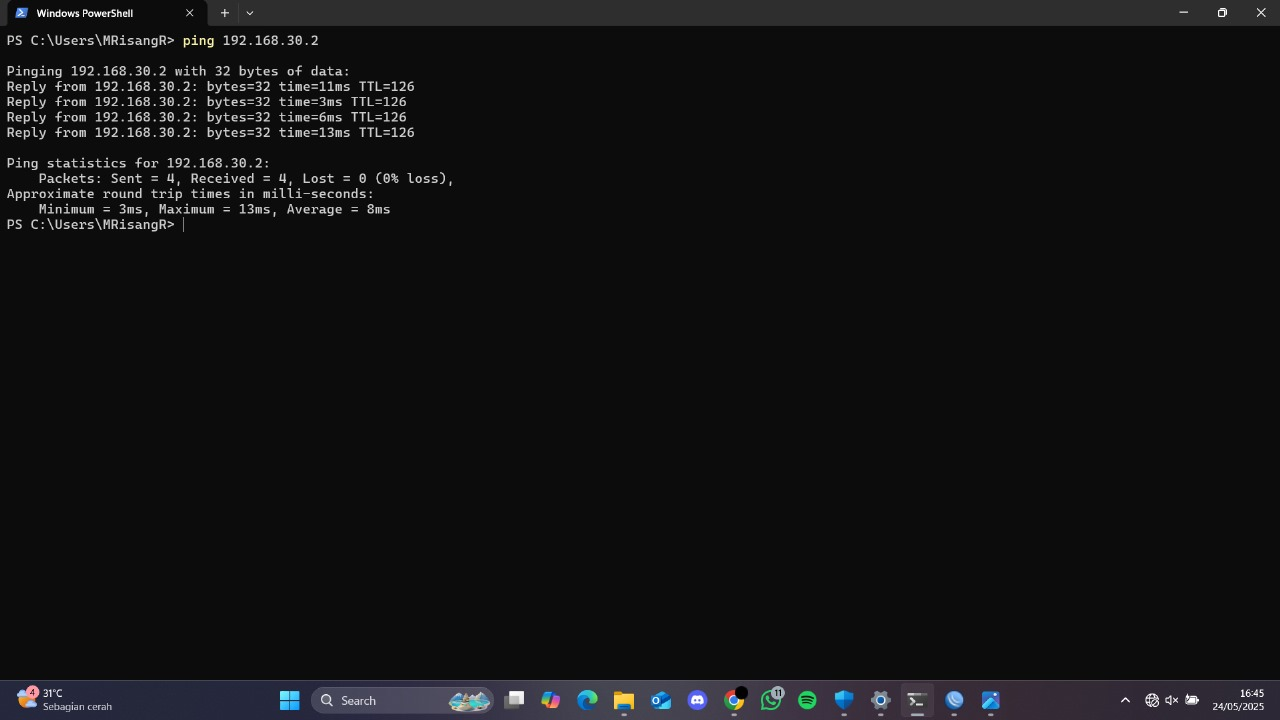
\includegraphics[width=\linewidth]{image/bridge11.jpg}
      \caption{Laptop 1}
    \end{subfigure}
    \hspace{1cm}
    \begin{subfigure}[b]{0.3\linewidth}
      \centering
      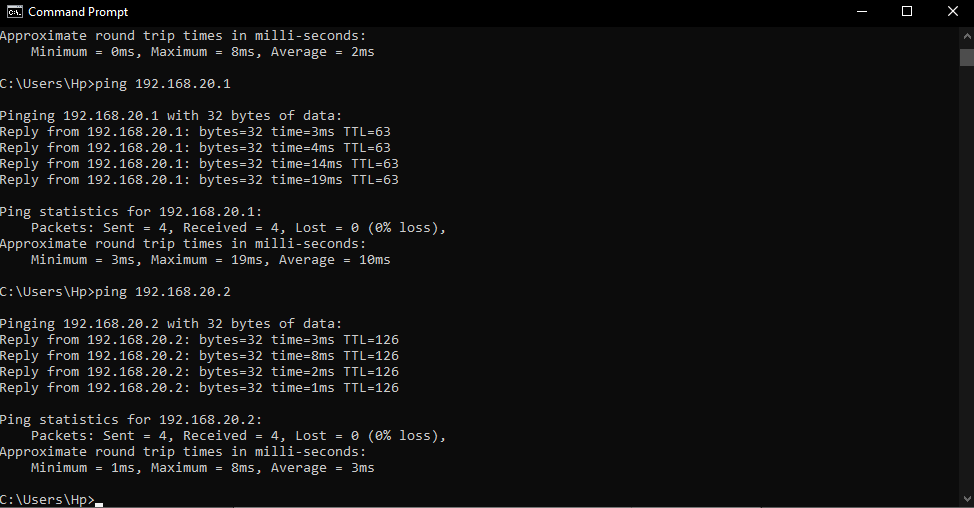
\includegraphics[width=\linewidth]{image/bridge9.png}
      \caption{Laptop 2}
    \end{subfigure}
    \caption{uji test ping cmd}
\end{figure}


\subsection{Wireles Point to Multipoint}
1. Aktifkan Interface Wireless Wlan 1 Masuk pada Menu Wireless-> Wifi Interface -> Klik interface Wlan 1 dan tekan tanda panah warna biru untuk enable Konfigurasikan untuk Router A Sebagai ( setelah double Klik pada interface wlan 1 masuk ke tab Wireless ) : Mode : Ap bridge ; SSID : PointToMultipoint 17.
\begin{figure}[H]
    \centering
    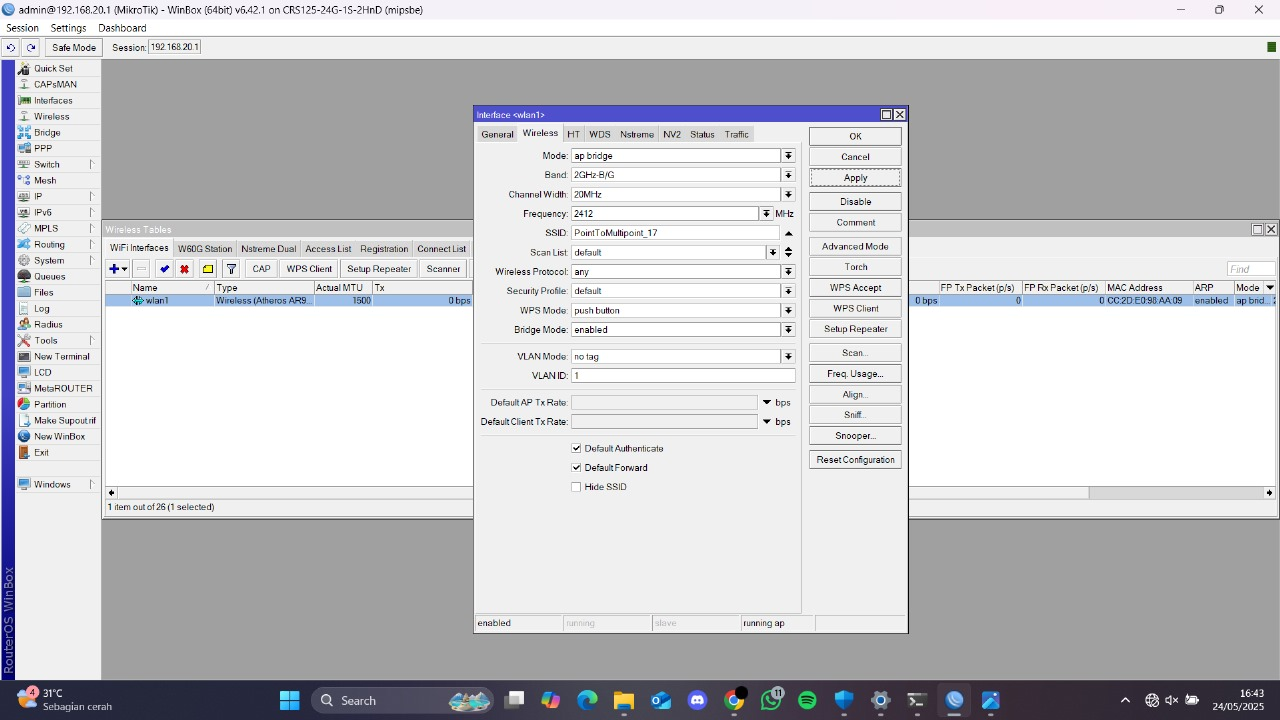
\includegraphics[width=0.65\linewidth]{image/station2.jpg}
    \label{fig:inirujukan}
    \caption{Konfigurasi router A}
\end{figure}
Konfigurasikan untuk Router B Sebagai ( setelah double Klik pada interface wlan 1 masuk ke tab Wireless ) : Mode : Station Bridge. Setelah itu klik tombol scan dan pilih interface menjadi wlan 1 lalu akan muncul berbagai jaringan wifi cari nama wifi yang sesuai dengan Router A lalu klik Connect.
\begin{figure}[H]
    \centering
    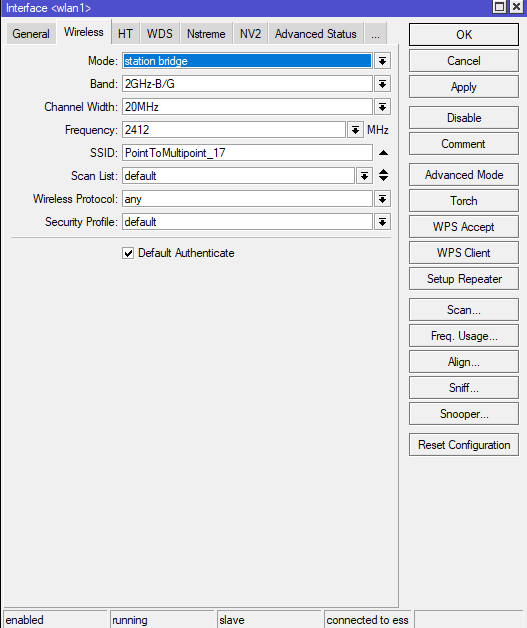
\includegraphics[width=0.65\linewidth]{image/station.png}
    \label{fig:inirujukan}
    \caption{Konfigurasi router B}
\end{figure}

2. Konfigurasi IP Address pada Wlan 1 Tambahkan IP address pada Wlan 1 yang digunakan sebagai jalur antar-router. Karena hanya ada dua perangkat yang terhubung (router A dan router B), IP Wlan 1 Router A : 10.10.10.1/29 ; IP Wlan 1 Router B : 10.10.10.2/29. \\
3. Konfigurasi IP Address untuk Jaringan LAN (note lakukan konfigurasi ini pada router A dan b) Tambahkan IP address pada ether 2 yang digunakan untuk menghubungkan Laptop dengan Router. IP ether 2 Router A : 192.168.20.1/24 ; IP ether 2 Router B : 192.168.30.1/24.
\begin{figure}[H]
    \centering
    \begin{subfigure}[b]{0.3\linewidth}
      \centering
      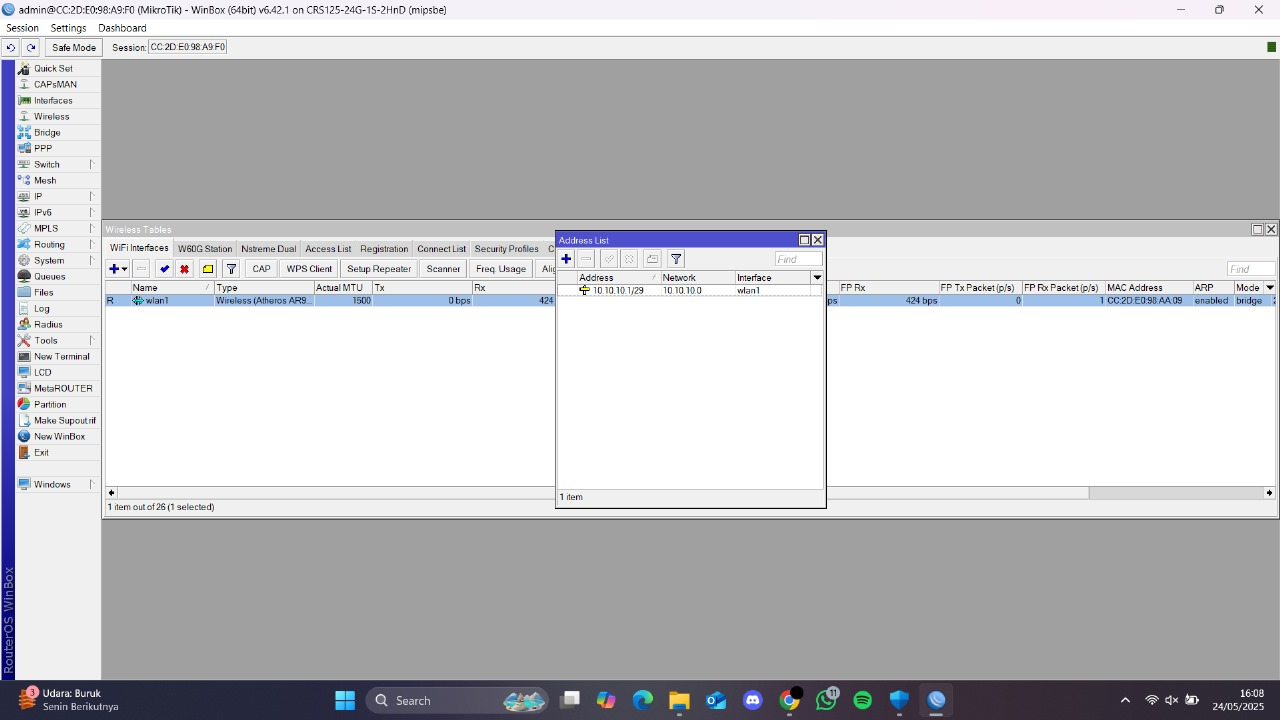
\includegraphics[width=\linewidth]{image/bridge4.jpg}
      \caption{router A}
    \end{subfigure}
    \hspace{1cm}
    \begin{subfigure}[b]{0.3\linewidth}
      \centering
      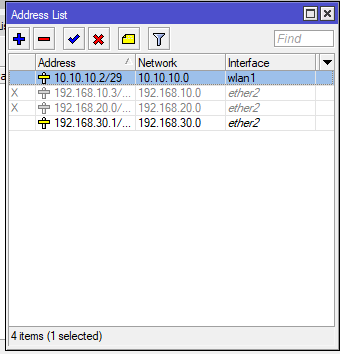
\includegraphics[width=\linewidth]{image/bridge1.png}
      \caption{router B}
    \end{subfigure}
    \caption{Konfigurasi Ip address wlan 1 dan ether 2}
\end{figure}

4. Konfigurasi Routing Statis (note lakukan konfigurasi ini pada router A dan b) Setelah semua interface diberi IP, langkah selanjutnya adalah menambahkan rute secara manual. Masuk ke menu IPv4 → Routes, kemudian klik "+" untuk menambahkan routing. Pada Router A, Dst. Address: 192.168.30.0/24 ; Gateway: 10.10.10.2. Pada Router B, Dst. Address: 192.168.20.0/24 ; Gateway: 10.10.10.1.
\begin{figure}[H]
    \centering
    \begin{subfigure}[b]{0.3\linewidth}
      \centering
      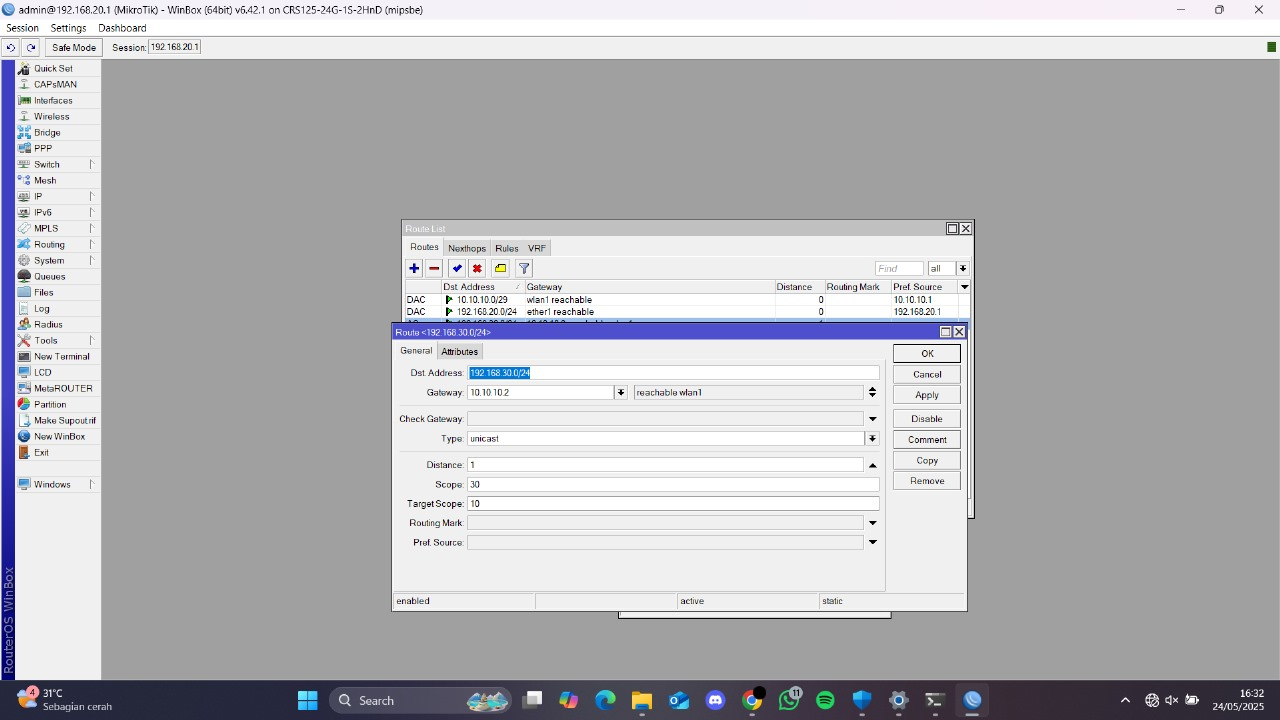
\includegraphics[width=\linewidth]{image/bridge6.jpg}
      \caption{router A}
    \end{subfigure}
    \hspace{1cm}
    \begin{subfigure}[b]{0.3\linewidth}
      \centering
      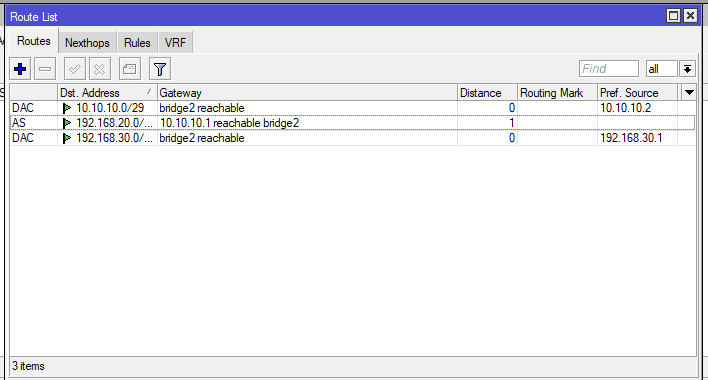
\includegraphics[width=\linewidth]{image/bridge3.png}
      \caption{router B}
    \end{subfigure}
    \caption{Konfigurasi routing statis}
\end{figure}

5. Test Koneksi Antar Router
\begin{figure}[H]
    \centering
    \begin{subfigure}[b]{0.3\linewidth}
      \centering
      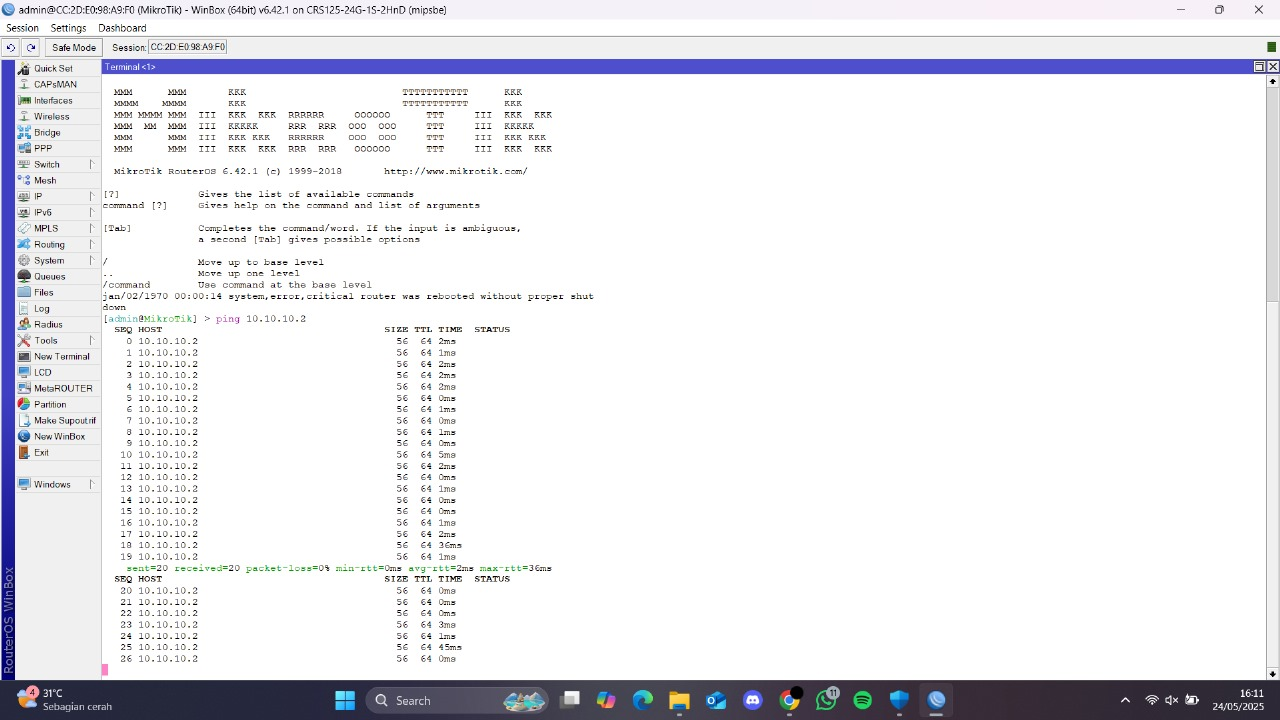
\includegraphics[width=\linewidth]{image/station3.jpg}
      \caption{router A}
    \end{subfigure}
    \hspace{1cm}
    \begin{subfigure}[b]{0.3\linewidth}
      \centering
      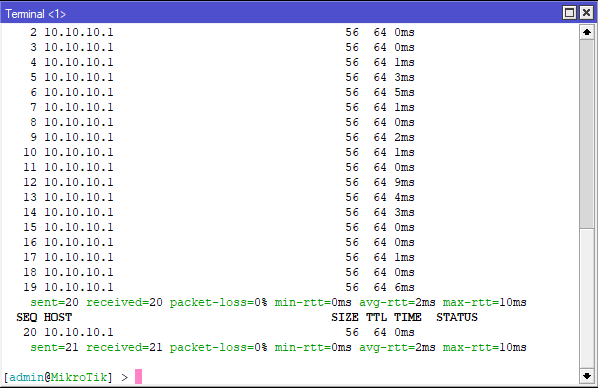
\includegraphics[width=\linewidth]{image/station1.png}
      \caption{router B}
    \end{subfigure}
    \caption{Ping terminal Winbox}
\end{figure}

6. Konfigurasi IP Adress di Laptop (note lakukan konfigurasi ini laptop yang terhubung pada router A dan b masing-masing) Karena ini masih menggunakan konfigurasi Static IP tambahkan IP address secara manual ke interface di laptop masing-masing bisa lewat Control Panel atau langsung di settings Windows, pastikan IP dan Gateway sudah benar sesuai Ether 2. Pada laptop yang terhubung ke Router A, IP Address : 192.168.20.2 ; Gateway : 192.168.20.1 (Router A) ; DNS : 8.8.8.8. Pada laptop yang terhubung ke Router B, IP Address: 192.168.30.2 ; Gateway : 192.168.30.1 (Router B) ; DNS : 8.8.8.8. 
\begin{figure}[H]
    \centering
    \begin{subfigure}[b]{0.3\linewidth}
      \centering
      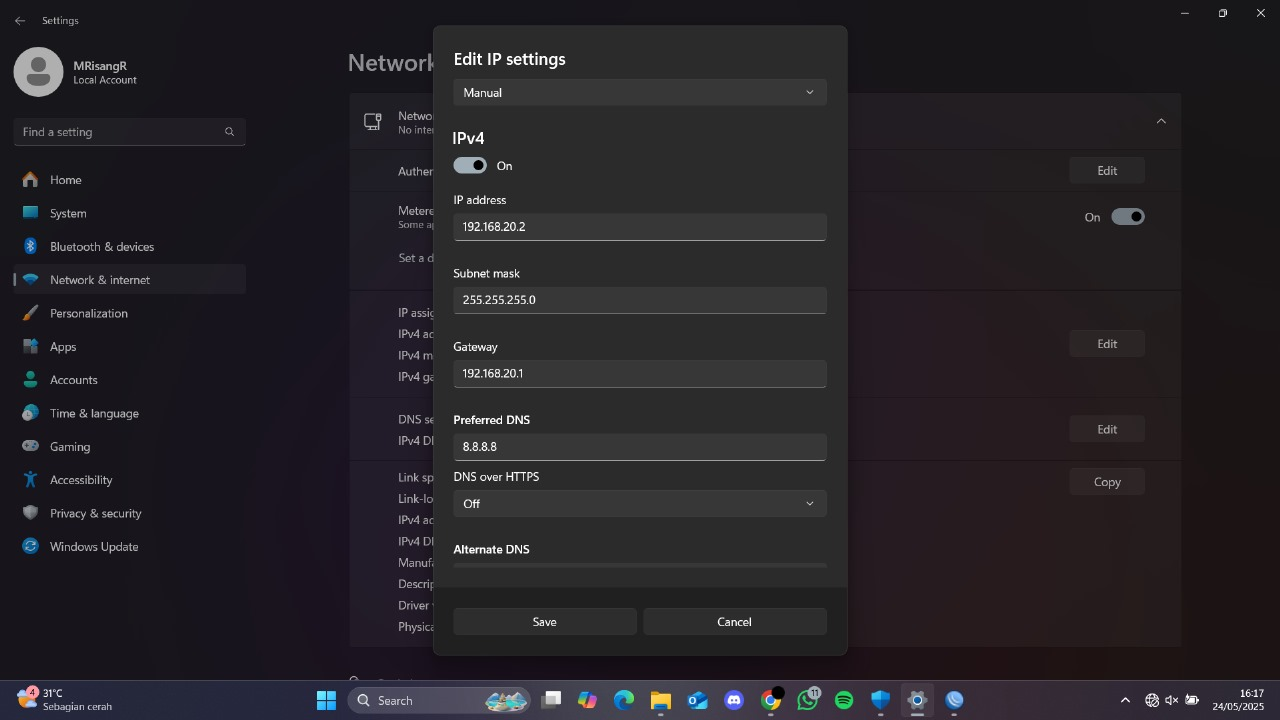
\includegraphics[width=\linewidth]{image/bridge10.jpg}
      \caption{Laptop 1}
    \end{subfigure}
    \hspace{1cm}
    \begin{subfigure}[b]{0.3\linewidth}
      \centering
      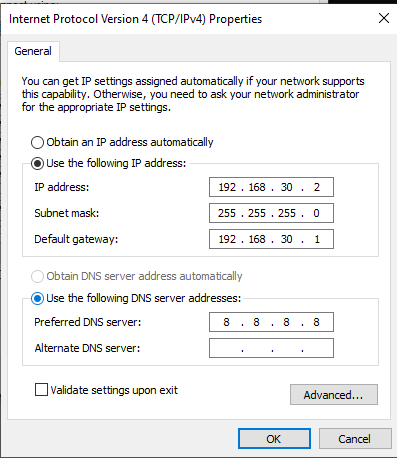
\includegraphics[width=\linewidth]{image/bridge7.png}
      \caption{Laptop 2}
    \end{subfigure}
    \caption{Ip address di masing-masing laptop}
\end{figure}

7. Jika Sudah Uji test PING dari Laptop 1 ke alamat Laptop 2, Jika berhasil maka Routing tidak ada masalah. Pada konfigurasikan Router B dan laptop yang terhubung ke Router B lakukan hal yang sama.
\begin{figure}[H]
    \centering
    \begin{subfigure}[b]{0.3\linewidth}
      \centering
      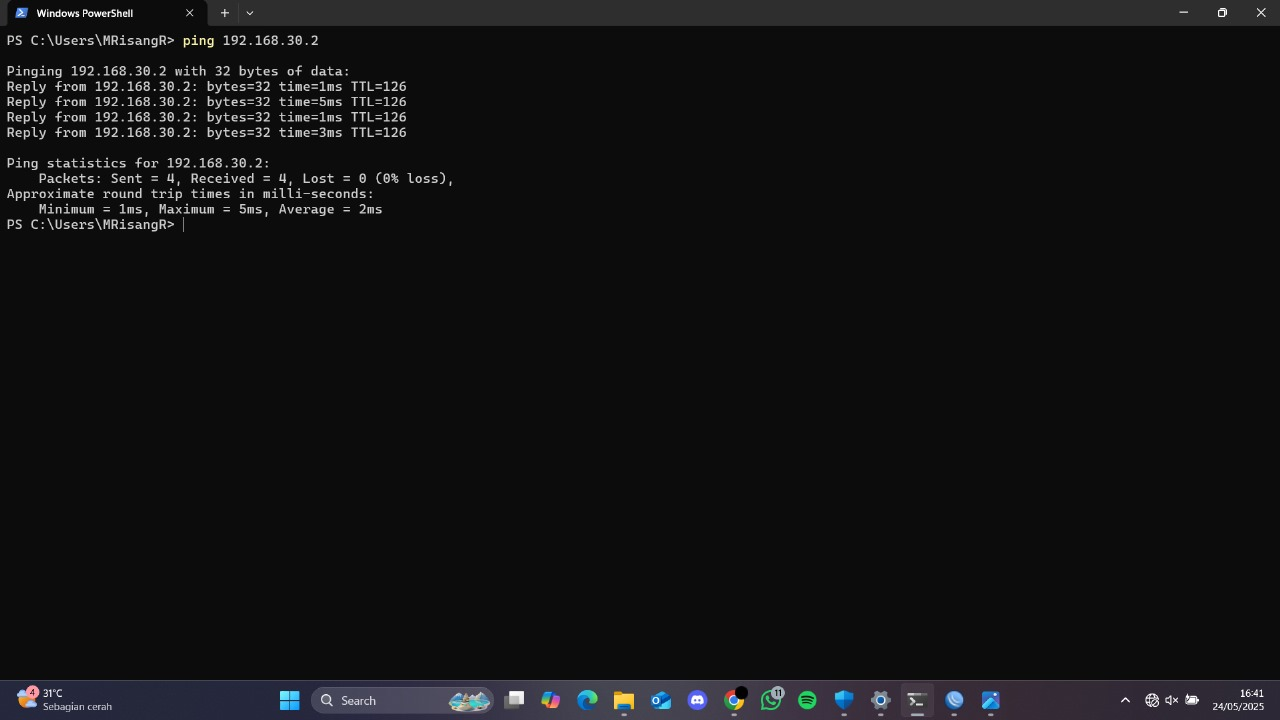
\includegraphics[width=\linewidth]{image/station4.jpg}
      \caption{Laptop 1}
    \end{subfigure}
    \hspace{1cm}
    \begin{subfigure}[b]{0.3\linewidth}
      \centering
      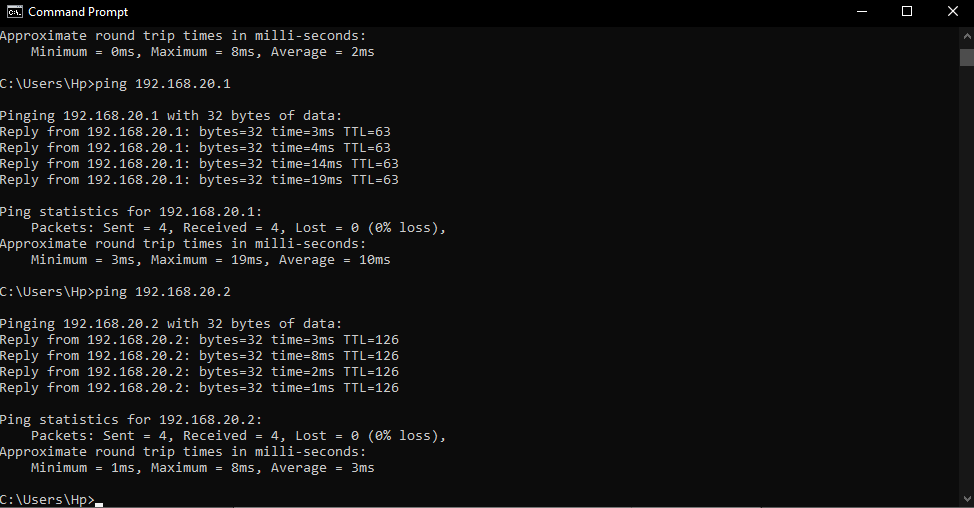
\includegraphics[width=\linewidth]{image/bridge9.png}
      \caption{Laptop 2}
    \end{subfigure}
    \caption{uji test ping cmd}
\end{figure}

\subsection{Wireless Bridge}
1. Aktifkan Interface Wireless Wlan 1 Masuk pada Menu Wireless-> Wifi Interface -> Klik interface Wlan 1 dan tekan tanda panah warna biru untuk enable Konfigurasikan untuk Router A Sebagai ( setelah double Klik pada interface wlan 1 masuk ke tab Wireless ) : Mode : Bridge ; SSID : WirelessBridge 17. 
\begin{figure}[H]
    \centering
    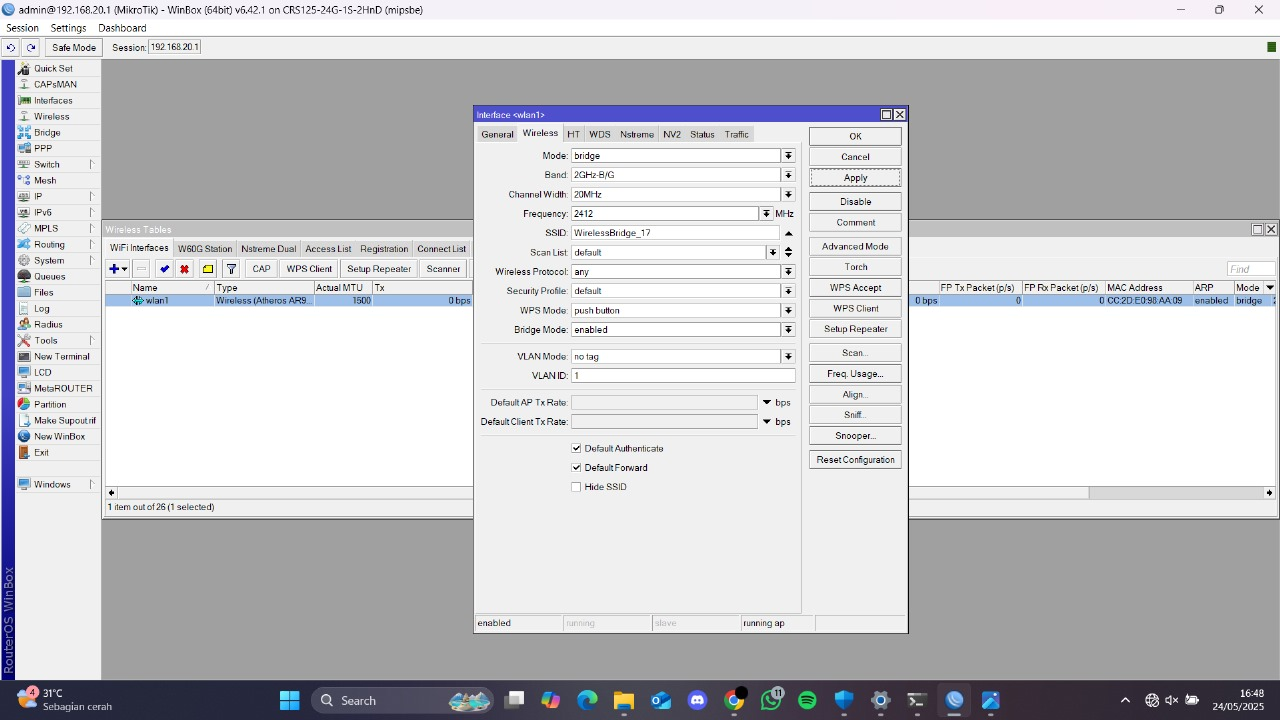
\includegraphics[width=0.65\linewidth]{image/wb2.jpg}
    \label{fig:inirujukan}
    \caption{Konfigurasi router A}
\end{figure}
Konfigurasikan untuk Router B Sebagai ( setelah double Klik pada interface wlan 1 masuk ke tab Wireless ) : Mode : Station Pseudobridge. Setelah itu klik tombol scan dan pilih interface menjadi wlan 1 lalu akan muncul berbagai jaringan wifi cari nama wifi yang sesuai dengan Router A lalu klik Connect.
\begin{figure}[H]
    \centering
    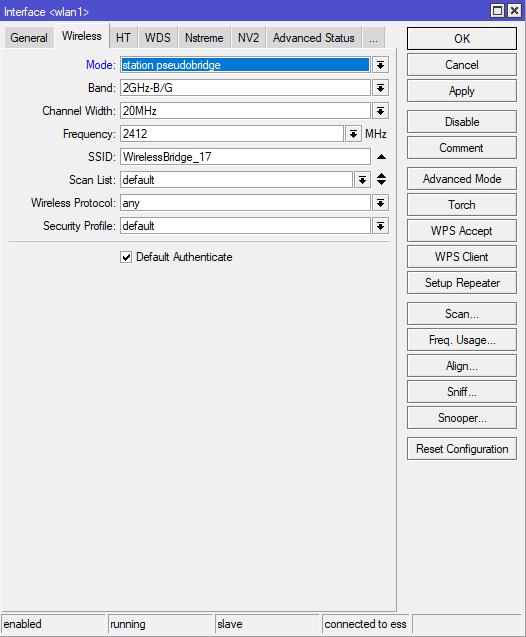
\includegraphics[width=0.65\linewidth]{image/wb.png}
    \label{fig:inirujukan}
    \caption{Konfigurasi router A}
\end{figure}

2. Konfigurasi IP Address pada Wlan 1 Tambahkan IP address pada Wlan 1 yang digunakan sebagai jalur antar-router. Karena hanya ada dua perangkat yang terhubung (router A dan router B), IP Wlan 1 Router A : 10.10.10.1/29 ; IP Wlan 1 Router B : 10.10.10.2/29. \\ 
3. Konfigurasi IP Address untuk Jaringan LAN (note lakukan konfigurasi ini pada router A dan b) Tambahkan IP address pada ether 2 yang digunakan untuk menghubungkan Laptop dengan Router. IP ether 2 Router A : 192.168.10.2/24 ; IP ether 2 Router B : 192.168.10.3/24.
\begin{figure}[H]
    \centering
    \begin{subfigure}[b]{0.3\linewidth}
      \centering
      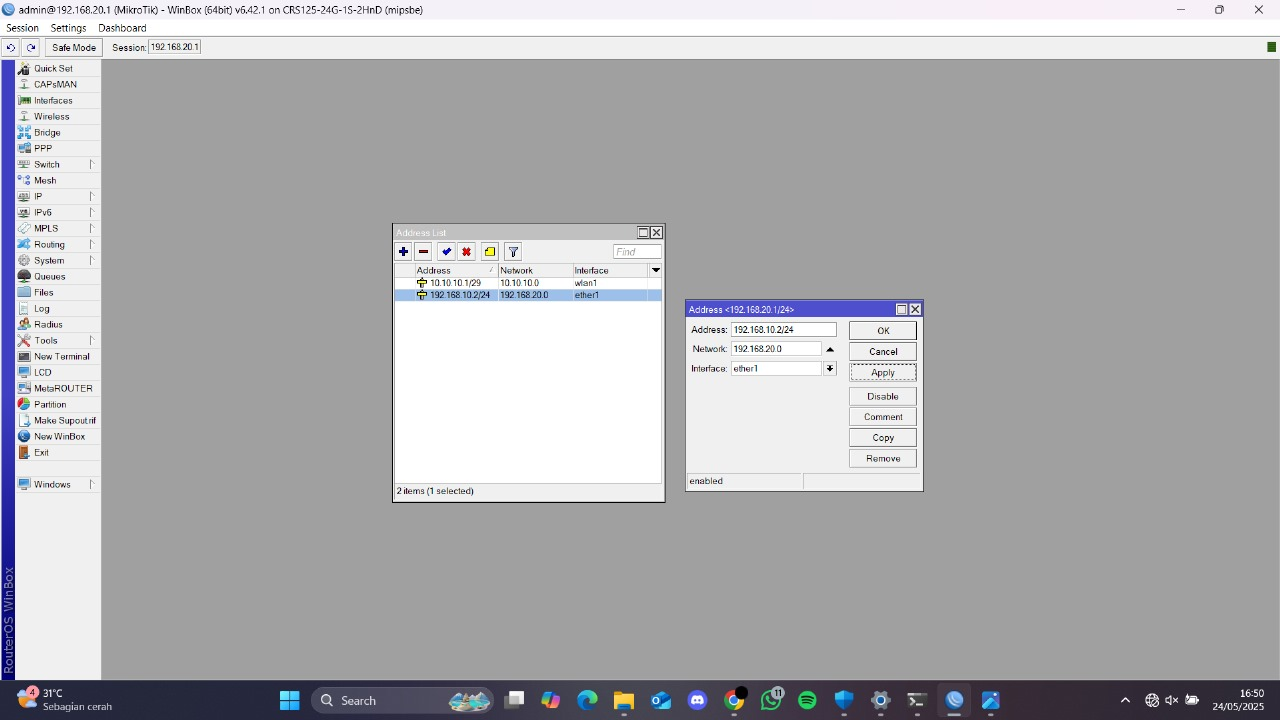
\includegraphics[width=\linewidth]{image/wb4.jpg}
      \caption{router A}
    \end{subfigure}
    \hspace{1cm}
    \begin{subfigure}[b]{0.3\linewidth}
      \centering
      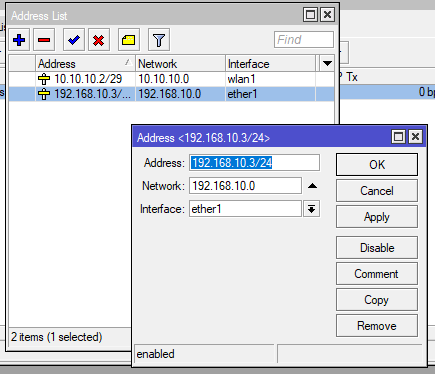
\includegraphics[width=\linewidth]{image/wb1.png}
      \caption{router B}
    \end{subfigure}
    \caption{Konfigurasi Ip address wlan 1 dan ether 2}
\end{figure}

4. Tambahkan bridge pada Router A dan B untuk menghubungkan wlan 1 dan ether 2 Router A : Masuk ke menu Bridge -> lalu tambah kan bridge dengan menekan tombol "+", lalu tambahkan untuk nama gunakan bridge1(atau yang lain). lalu masuk ke tab Port dan tambahkan : Interface Wlan 1 dan Ether 2 lalu gunakan bridge yang sudah di buat. \\ 
5. Test Koneksi Antar Router. \\
6.Konfigurasi IP Adress di Laptop (note lakukan konfigurasi ini laptop yang terhubung pada router A dan b masing-masing) Karena ini masih menggunakan konfigurasi Static IP tambahkan IP address secara manual ke interface di laptop masing-masing bisa lewat Control Panel atau langsung di settings Windows, pastikan IP dan Gateway sudah benar sesuai Ether 2. Pada laptop yang terhubung ke Router A, IP Address : 192.168.10.5 ; Gateway : 192.168.10.2 (Router A) ; DNS : 8.8.8.8. Pada laptop yang terhubung ke Router B, IP Address: 192.168.10.7 ; Gateway : 192.168.10.3 (Router B) ; DNS : 8.8.8.8
\begin{figure}[H]
    \centering
    \begin{subfigure}[b]{0.3\linewidth}
      \centering
      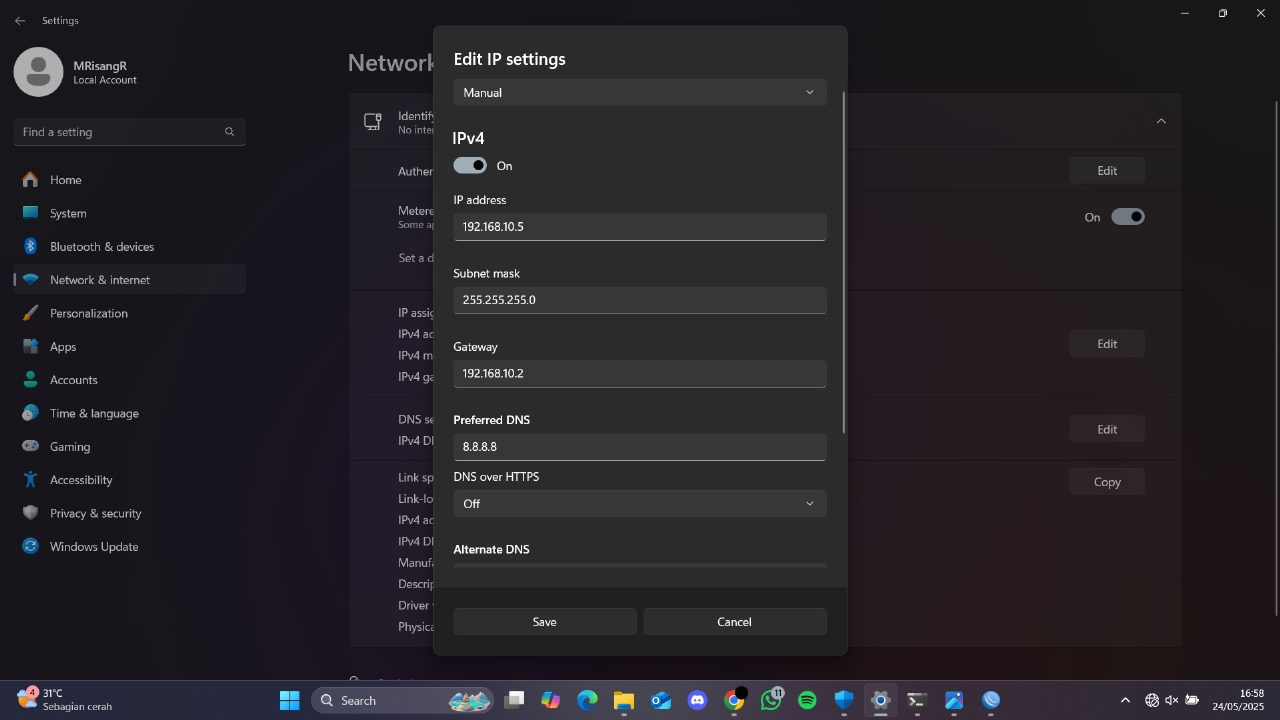
\includegraphics[width=\linewidth]{image/wb6.jpg}
      \caption{Laptop 1}
    \end{subfigure}
    \hspace{1cm}
    \begin{subfigure}[b]{0.3\linewidth}
      \centering
      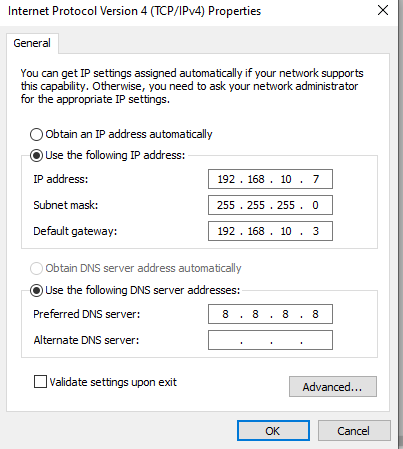
\includegraphics[width=\linewidth]{image/wb3.png}
      \caption{Laptop 2}
    \end{subfigure}
    \caption{Ip address di masing-masing laptop}
\end{figure}
7. Jika Sudah Uji test PING dari Laptop 1 ke alamat Laptop 2, Jika berhasil maka Routing tidak ada masalah. Pada konfigurasikan Router B dan laptop yang terhubung ke Router B lakukan hal yang sama
\begin{figure}[H]
    \centering
    \begin{subfigure}[b]{0.3\linewidth}
      \centering
      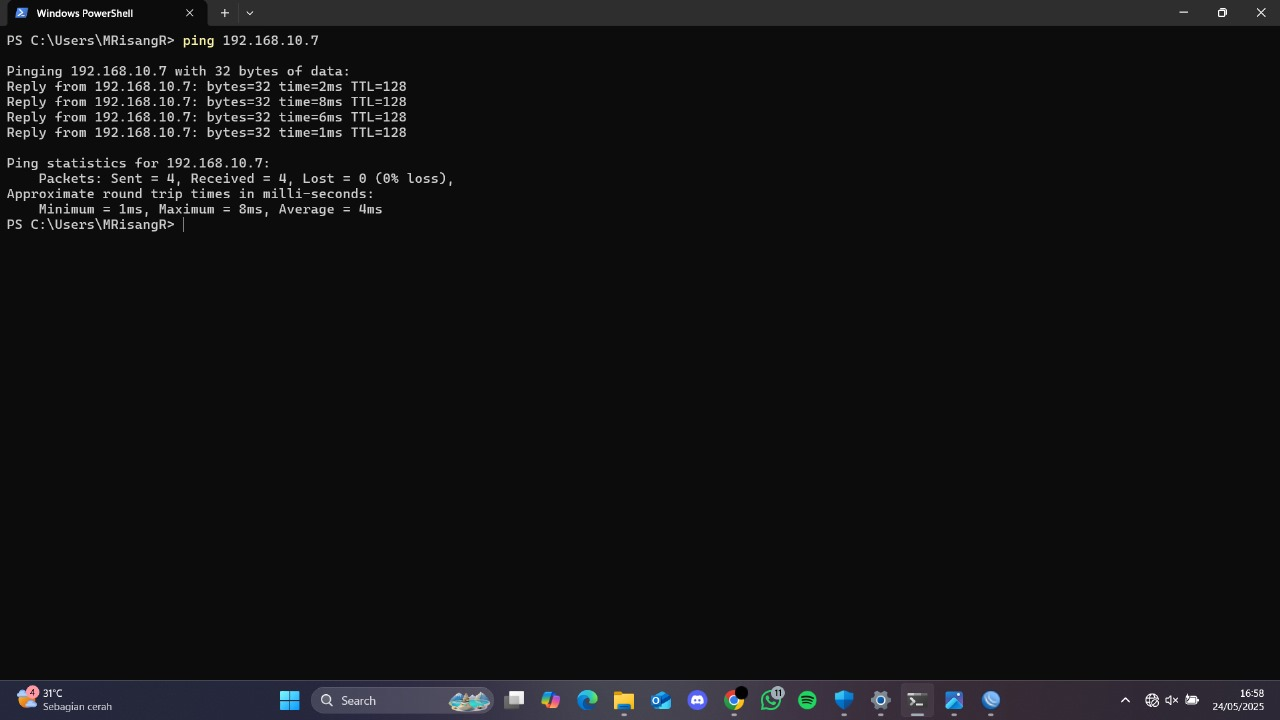
\includegraphics[width=\linewidth]{image/wb7.jpg}
      \caption{Laptop 1}
    \end{subfigure}
    \hspace{1cm}
    \begin{subfigure}[b]{0.3\linewidth}
      \centering
      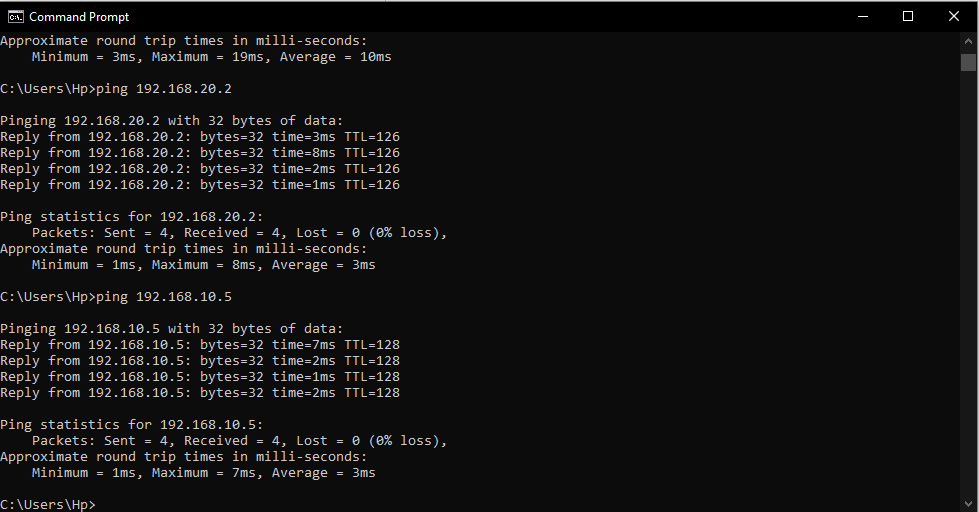
\includegraphics[width=\linewidth]{image/wb5.png}
      \caption{Laptop 2}
    \end{subfigure}
    \caption{uji test ping cmd}
\end{figure}

\section{Analisis Hasil Percobaan}
Hasil praktikum jaringan wireless yang meliputi konfigurasi Wireless Point-to-Point, Point-to-Multipoint, dan Wireless Bridge menunjukkan bahwa konsep dan implementasi jaringan nirkabel dapat diterapkan dengan baik sesuai teori. Dalam setiap skenario, praktikan berhasil menghubungkan dua atau lebih router menggunakan interface wireless dan mengatur konektivitas antar perangkat melalui pengujian ping, yang menjadi indikator utama bahwa jaringan telah terkonfigurasi dengan benar. Hasil ini sesuai dengan prinsip dasar teori, di mana mode wireless seperti bridge, station, dan AP bridge memainkan peran penting dalam membangun hubungan komunikasi antar perangkat. Keberhasilan konfigurasi IP address dan routing statis menunjukkan bahwa praktikan memahami pentingnya pengalamatan yang benar dan peran routing dalam komunikasi lintas jaringan. \\ Namun demikian, terdapat beberapa faktor yang dapat memengaruhi hasil percobaan. Pada saat praktikum lupa untuk mematikan salah satu firewall yang menghabiskan waktu lumayan lama, dan juga masalah pada kabel LAN yang tidak begitu efektif. Melalui praktikum ini, praktikan diharapkan mampu mengevaluasi konfigurasi jaringan secara mandiri dan memahami peran masing-masing perangkat wireless dalam membangun jaringan yang efisien, fleksibel, dan aman tanpa kabel.

\section{Hasil Tugas Modul}

\section{Kesimpulan}
Praktikum jaringan wireless berhasil dilaksanakan dengan tiga skenario utama: Wireless Point-to-Point, Point-to-Multipoint, dan Wireless Bridge. Tujuan praktikum, yaitu memahami dan mengimplementasikan jaringan nirkabel antar perangkat menggunakan konfigurasi yang sesuai dengan kebutuhan topologi, telah tercapai dengan baik. Praktikan mampu mengonfigurasi mode wireless pada router, memberikan IP address yang tepat, serta menambahkan routing statis agar perangkat dalam jaringan yang berbeda dapat saling berkomunikasi. Hasil yang diperoleh secara umum sesuai dengan teori yang dipelajari, di mana masing-masing perangkat berfungsi sebagaimana mestinya untuk membangun konektivitas jaringan tanpa kabel. \\ Praktikum ini juga memberikan wawasan penting terkait faktor-faktor yang memengaruhi keberhasilan jaringan wireless, seperti ketelitian konfigurasi, pemilihan mode, dan penyesuaian IP yang tepat. Praktikan juga belajar mengidentifikasi dan menyelesaikan masalah umum yang muncul saat implementasi, seperti kesalahan IP atau kegagalan koneksi antar interface. Dengan demikian, praktikum ini tidak hanya memperkuat pemahaman konsep jaringan wireless, tetapi juga melatih kemampuan troubleshooting dan analisis dalam penerapan jaringan di dunia nyata.

\section{Lampiran}
\begin{figure}[H]
    \centering
    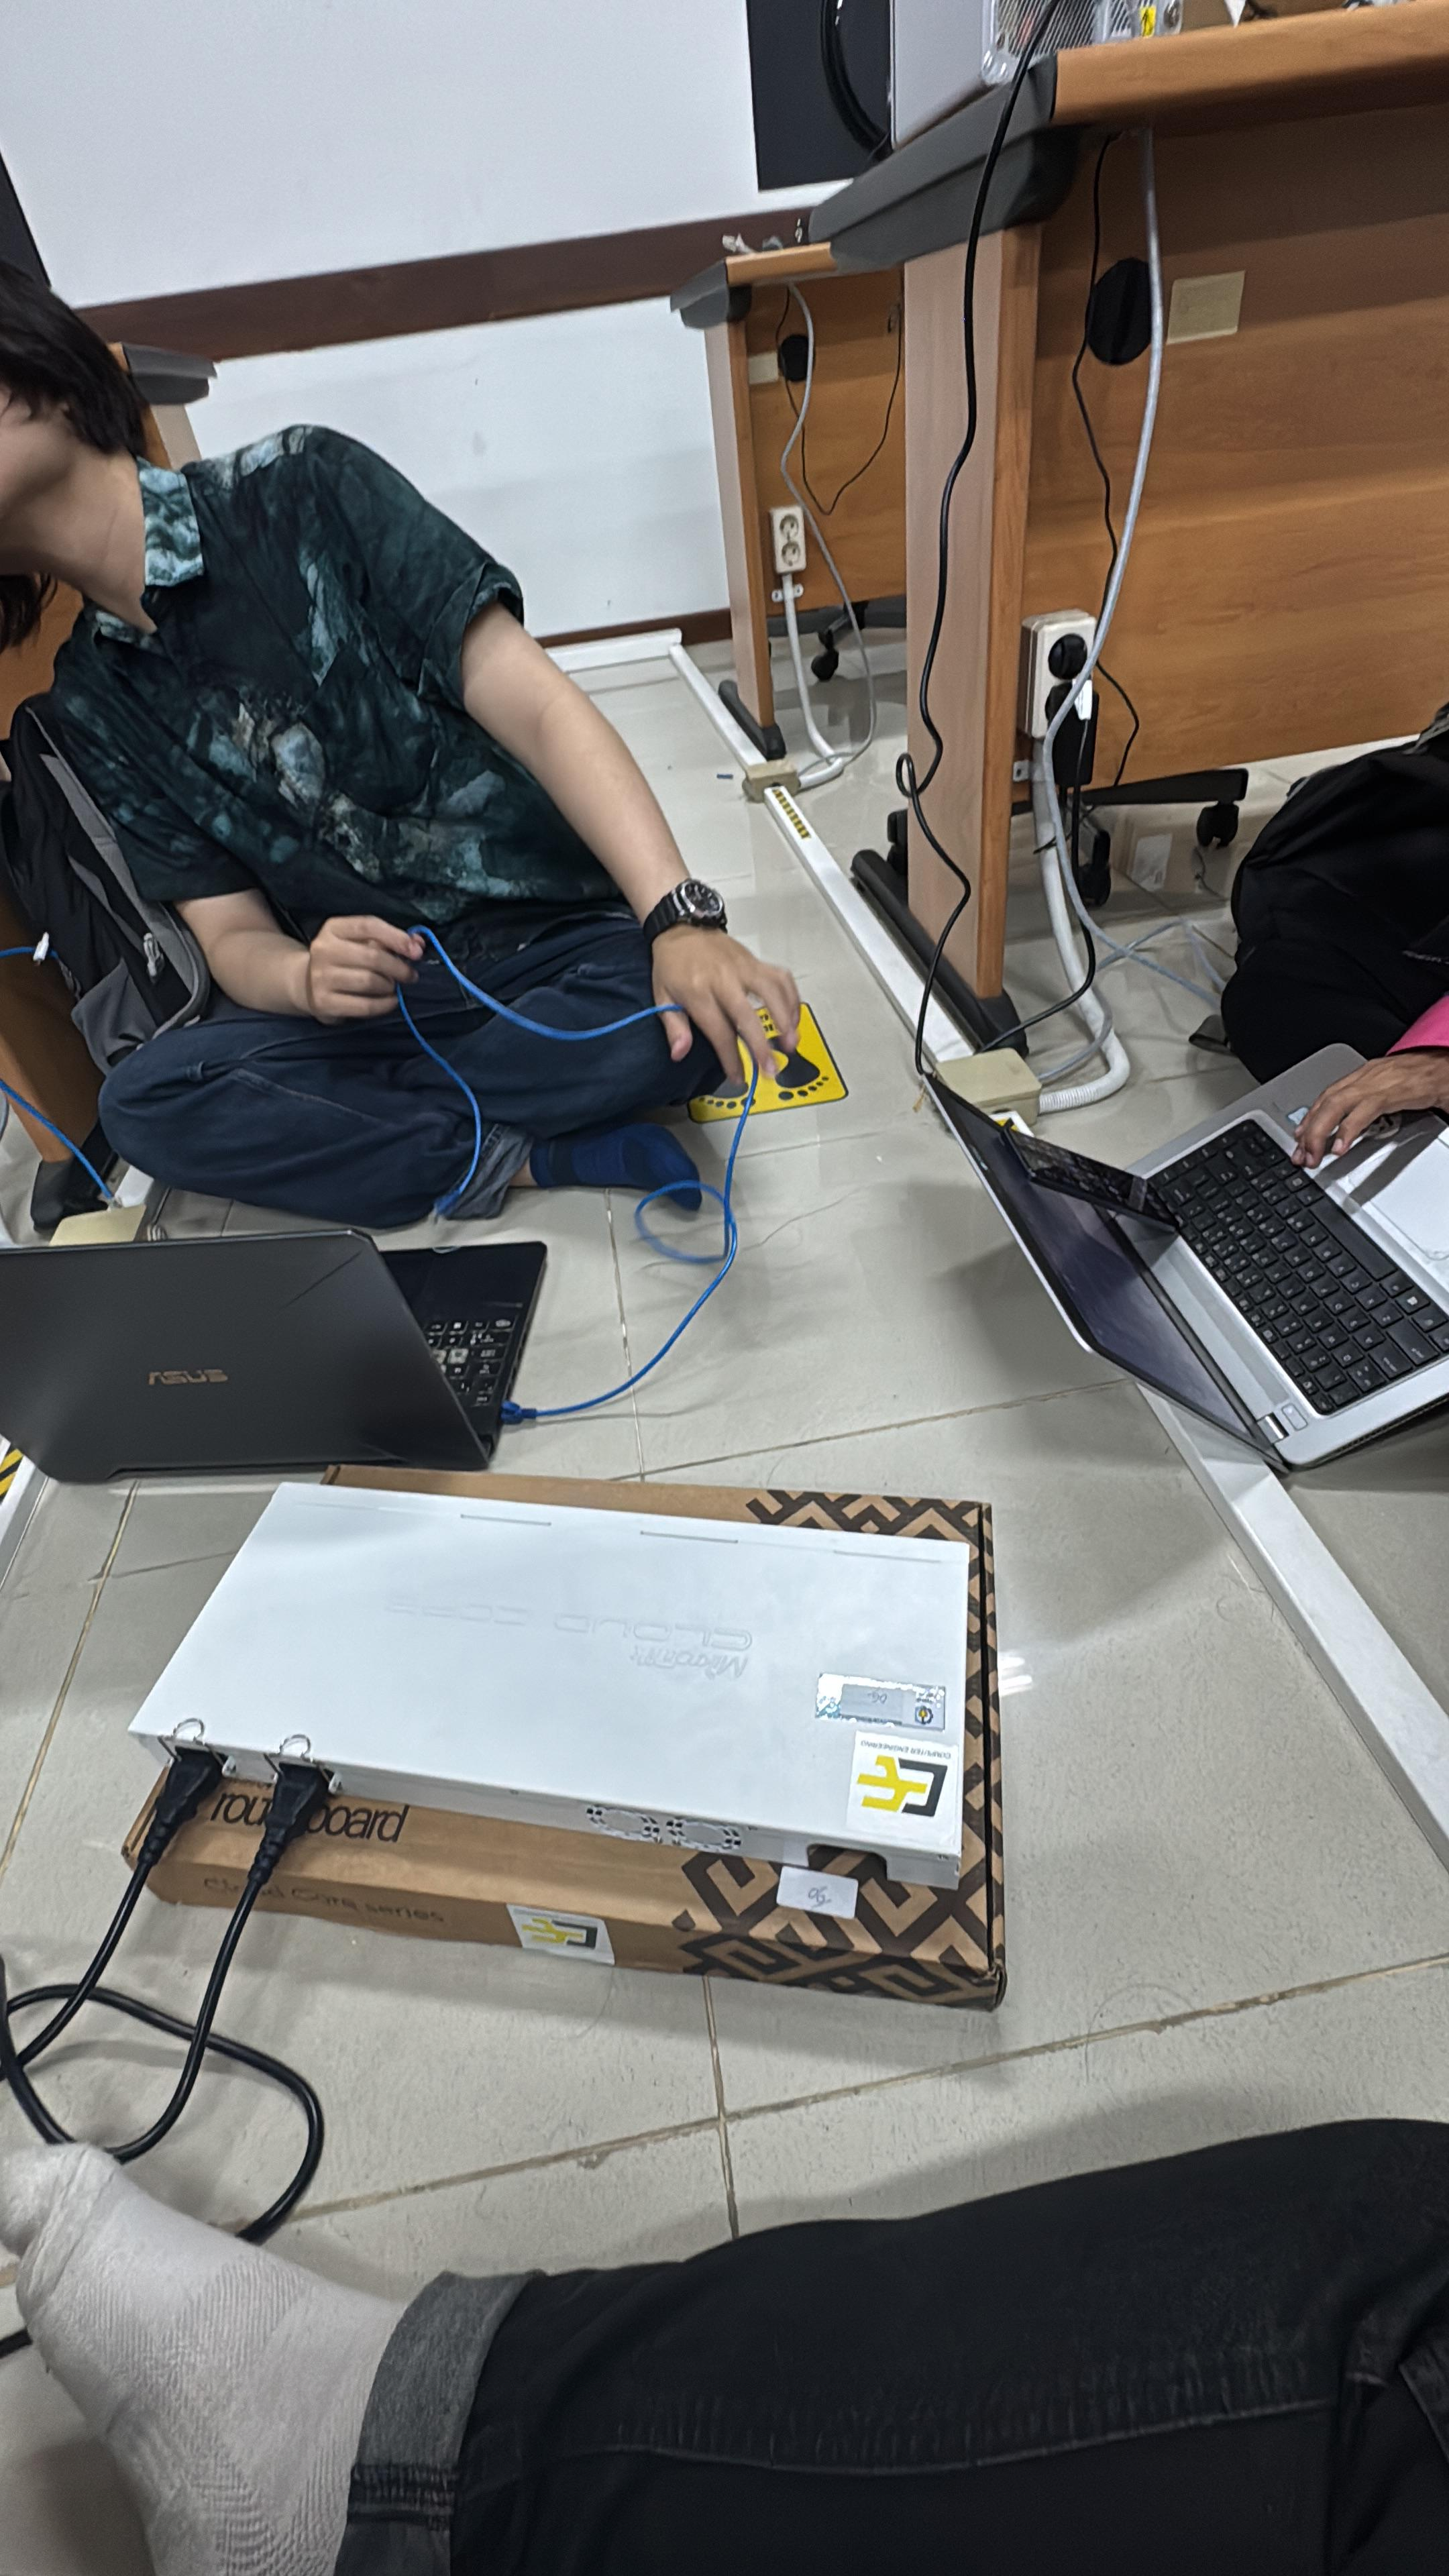
\includegraphics[width=0.65\linewidth]{image/dokum.jpg}
    \label{fig:inirujukan}
\end{figure}


\end{document}